\documentclass[conference]{IEEEtran}
\IEEEoverridecommandlockouts

\usepackage{cite}
\usepackage{amsmath,amssymb,amsfonts}
\usepackage{algorithmic}
\usepackage{graphicx}
\usepackage{textcomp}
\usepackage{xcolor}
\usepackage{booktabs}
\usepackage{array}
\usepackage{url}

\def\BibTeX{{\rm B\kern-.05em{\sc i\kern-.025em b}\kern-.08em
    T\kern-.1667em\lower.7ex\hbox{E}\kern-.125emX}}

\begin{document}

\title{An Explainable Multi-Stage Decision-Support Pipeline for Chest X-Ray Classification, Localization, and Structured Reporting}

\author{\IEEEauthorblockN{Sri Datta Ganesh Bandreddi}
\IEEEauthorblockA{\textit{Biomedical Engineering} \\
\textit{Carnegie Mellon University}\\
Pittsburgh, PA, USA \\
sbandred@andrew.cmu.edu}
}

\maketitle

\begin{abstract}
When a radiologist reviews a chest X-ray, the cognitive task is not a single classification: it involves identifying which findings are present, locating the supporting image evidence, and synthesizing those observations into a communicable impression. Most automated chest X-ray systems target only the first step and return a probability vector that is difficult for a downstream clinician to interpret or audit. This work addresses the full decision-support loop by constructing a three-stage pipeline on a 15-label publicly available subset of the VinBigData chest X-ray dataset. The first stage performs multi-label image classification, where transfer-learned models are strongest and a Swin Transformer achieves a macro AUC-ROC of 0.9665, while a lightweight 1.31M-parameter CNN trained from scratch remains competitive at 0.9314 for lighter compute settings. The second stage provides spatial evidence through YOLOv8m bounding-box localization (0.3666 mAP@0.5). The third stage is an agentic reporting layer that consumes both classifier probabilities and detector outputs and produces a structured summary containing supported findings, uncertain findings, and explicit review guidance. On a 300-case evaluation, the integrated workflow reaches 0.750 exact-match accuracy and 0.9560 macro accuracy. The principal contribution is the pipeline architecture itself: a modular, auditable workflow in which each stage can be inspected, replaced, or refined independently, designed to serve as a first-pass clinical decision-support tool rather than a standalone diagnostic system.
\end{abstract}

\begin{IEEEkeywords}
Chest X-ray, VinBigData, multi-label classification, Swin Transformer, YOLOv8, explainable AI, clinical decision support, structured reporting.
\end{IEEEkeywords}

\section{Introduction}
Chest radiography accounts for roughly 40\% of all diagnostic imaging worldwide, and that volume makes it a natural target for machine learning assistance. However, the clinical value of an automated system depends less on classification accuracy in isolation than on whether it fits the way radiologists actually work. A radiologist reading a chest X-ray performs several interleaved tasks: screening for abnormalities, localizing the anatomical basis for each finding, assessing confidence in the evidence, and composing a structured impression that another clinician can act on. Most existing automated systems address only the first task, image-level classification, and stop at a probability vector that is opaque to the downstream user.

This gap between model output and clinical usability motivates the present work. Rather than optimizing a single classification metric, the project constructs a multi-stage pipeline that mirrors the radiologist's cognitive workflow:
\begin{enumerate}
    \item \textbf{Classification}: determining which of 15 abnormality labels are present.
    \item \textbf{Localization}: providing bounding-box evidence that shows \textit{where} in the image the findings are supported.
    \item \textbf{Structured reporting}: synthesizing the classification and localization outputs into a concise, auditable summary that distinguishes confident findings from uncertain ones and flags classifier-detector disagreement.
\end{enumerate}

The design goal is not diagnostic autonomy. Instead, the system is intended as a first-pass assistant: a tool that organizes the evidence so that a clinician can review it faster, with explicit visibility into what the model found, where it found it, and how confident each component is. Each pipeline stage is independently replaceable, so the workflow can evolve as better classifiers, detectors, or report generators become available.

The work makes three practical contributions: a reproducible classifier benchmark showing the value of transfer learning on the public VinBigData subset while retaining a lightweight from-scratch alternative for low-compute settings; a YOLOv8m localization branch that provides spatial supporting evidence; and an agentic reporting layer that merges classifier and detector outputs into a structured decision-support summary.

\begin{figure*}[t]
\centering
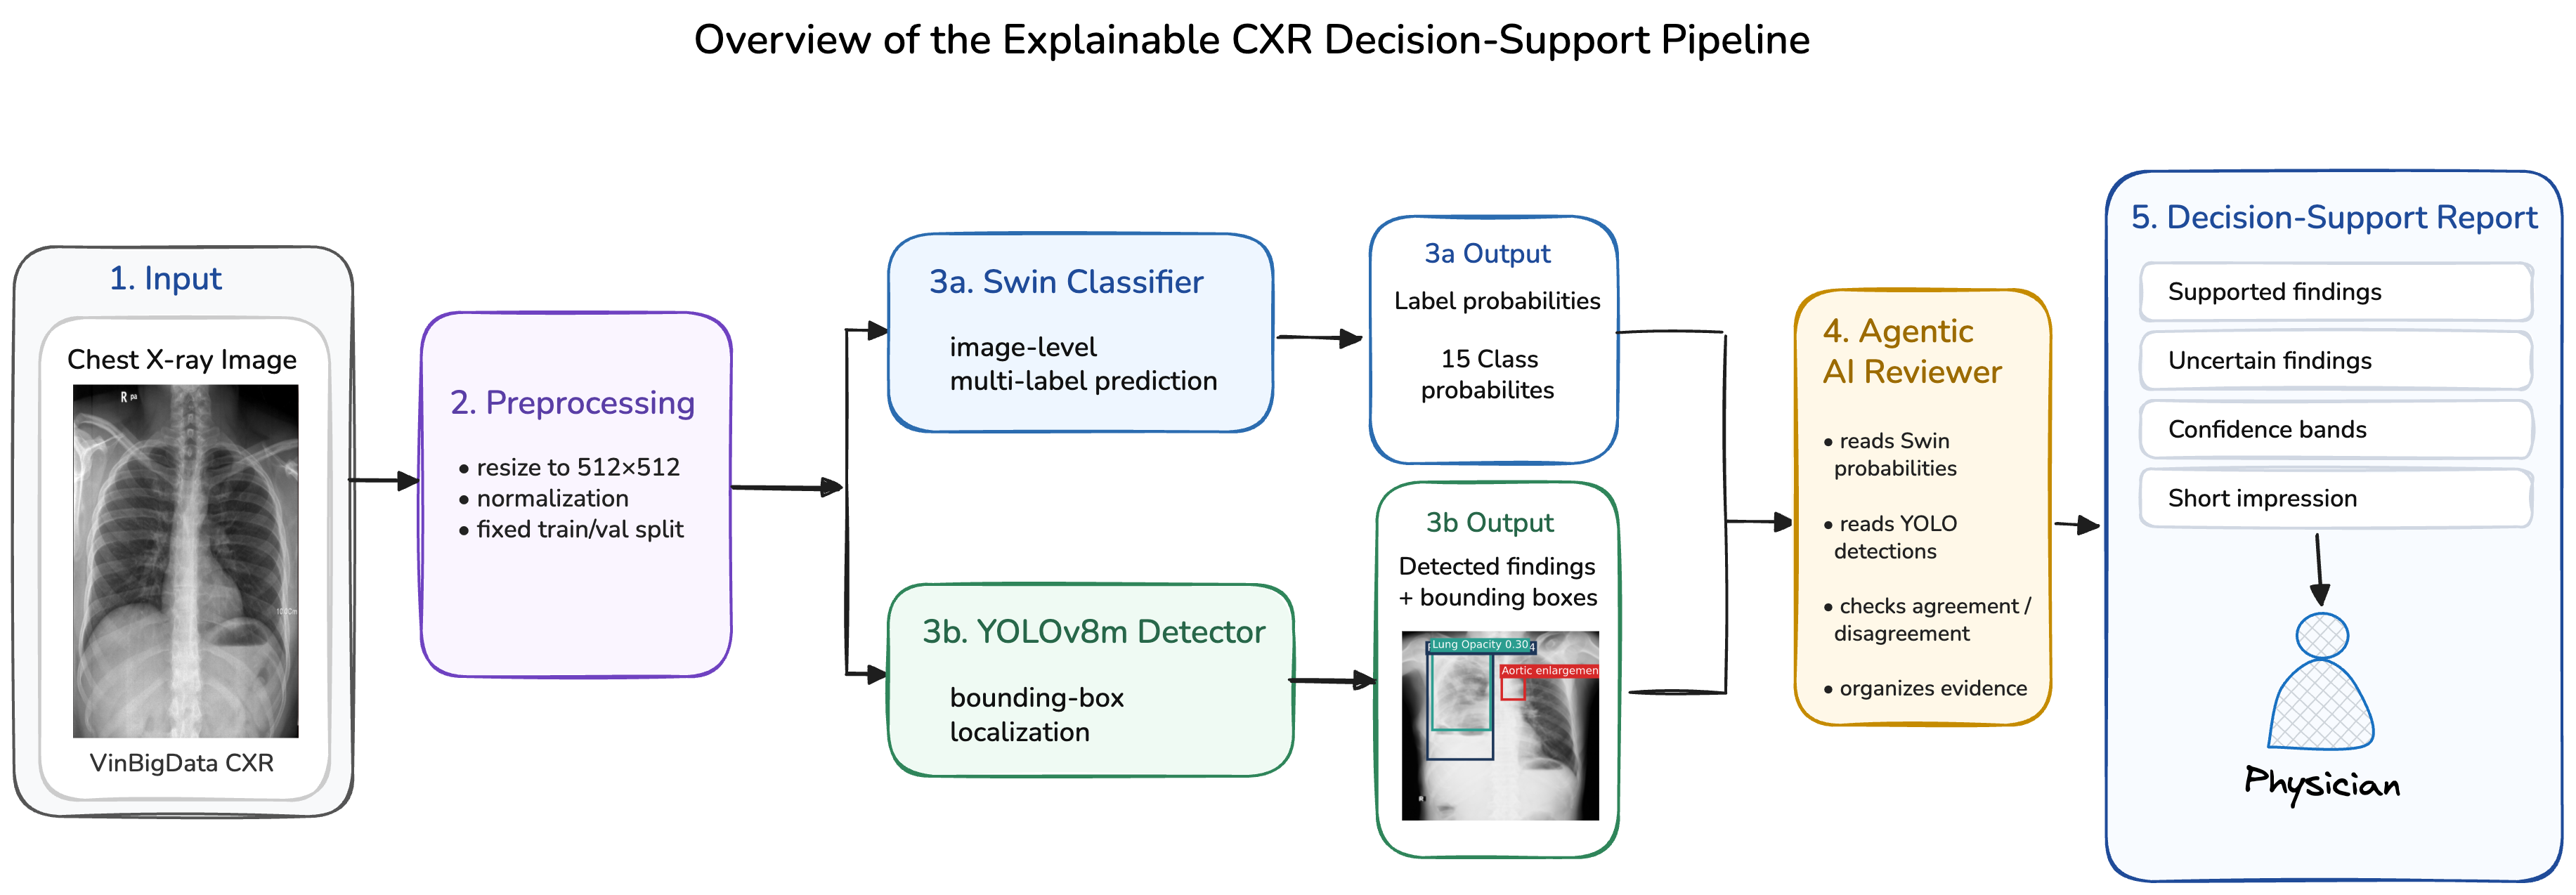
\includegraphics[width=0.9\textwidth]{figures/pipeline_abstract.png}
\caption{Locked workflow used in the final repository: chest X-ray image, Swin classification, YOLO localization support, and agentic AI report generation.}
\label{fig:pipeline}
\end{figure*}

\section{Related Work}
Prior work on chest X-ray AI has addressed classification, localization, and report generation largely as separate research threads. CheXNet showed that a DenseNet trained on ChestX-ray14 could match radiologist-level sensitivity for pneumonia detection, establishing deep transfer learning as the dominant approach for image-level classification \cite{chexnet}. Pham et al.\ extended this to the VinDr-CXR dataset by pairing multi-label classification with lesion localization and demonstrating that the combined output improved inter-reader agreement, providing early evidence that localization support has direct clinical utility \cite{pham2022vindr}.

On the report-generation side, approaches have ranged from fine-grained label conditioning \cite{syedamahmood2020finegrained} and contrastive attention \cite{liu2021contrastive} to variational topic inference \cite{najdenkoska2022uncertainty}. More recently, multimodal LLMs such as CXR-LLaVA \cite{lee2023cxrllava} and GPT-4-based impression generators \cite{ziegelmayer2023gpt4} have shown that large vision-language models can produce readable chest X-ray summaries. However, these systems are typically trained end-to-end on large report corpora (e.g., MIMIC-CXR) and treat the report as a single monolithic output, making it difficult to attribute a specific sentence in the generated text to a specific visual finding or model decision.

The present work addresses a different design point. Instead of training a single end-to-end model, it assembles a modular pipeline from a bounded VinBigData subset with image-level labels and localization annotations, keeping the classifier, detector, and reporting stages explicitly separable. This modularity is the key architectural distinction: each stage's output is visible and auditable, so a clinician reviewing the final summary can trace any stated finding back to a classifier probability, a detector bounding box, or a disagreement between the two. The trade-off is clear. This approach does not benefit from joint end-to-end training, but it gains transparency and component-level replaceability that matter in a clinical decision-support setting.

\section{Dataset and Task Formulation}
The pipeline operates on the publicly available Kaggle release of the VinBigData chest X-ray dataset, using the 15-label setup exposed by that competition. This public release is a truncated view of the broader original labeling space: in practice, the clinical findings contain both more local findings that admit spatial support and more global or report-level categories that do not map as cleanly to a single focal box. Even with that truncation, the public dataset remains an excellent proxy for the intended pipeline because it still contains a useful mix of localizable findings, diffuse findings, and the global \textit{No finding} category.

The retained labels span a clinically meaningful range: \textit{Aortic enlargement}, \textit{Atelectasis}, \textit{Calcification}, \textit{Cardiomegaly}, \textit{Consolidation}, \textit{ILD}, \textit{Infiltration}, \textit{Lung Opacity}, \textit{Nodule/Mass}, \textit{Other lesion}, \textit{Pleural effusion}, \textit{Pleural thickening}, \textit{Pneumothorax}, \textit{Pulmonary fibrosis}, and \textit{No finding}. Because a single radiograph may present multiple concurrent abnormalities, for example cardiomegaly alongside pleural effusion, the image-level task is formulated as multi-label classification rather than single-label assignment.

The localization task uses the raw VinBigData bounding-box annotations to train a YOLOv8m detector. These annotations are not an afterthought: the boxes are provided explicitly in the public release for abnormal findings, which makes it possible to preserve image-level labels and spatial labels in a consistent pipeline. Importantly, the classification and localization tasks are evaluated separately because they answer different clinical questions. Classification addresses \textit{what} abnormalities are present anywhere in the image; localization addresses \textit{where} the spatially plausible supporting evidence lies. The two streams are connected only in the downstream reporting stage, where agreement or disagreement between them becomes an explicit signal of confidence.

From an EDA standpoint, the public labeled portion provides 15,000 studies, and this repository uses a fixed split of 12,000 training images and 3,000 validation images. That split is reused across all experiments to ensure that performance differences reflect model choices rather than data sampling. The dataset is also visibly imbalanced: \textit{No finding} is common, several chronic or diffuse abnormalities are relatively rare, and the frequency distribution is long-tailed. This is precisely why the dataset is useful for evaluating an auditable pipeline rather than a single closed classifier.

\begin{figure}[t]
\centering
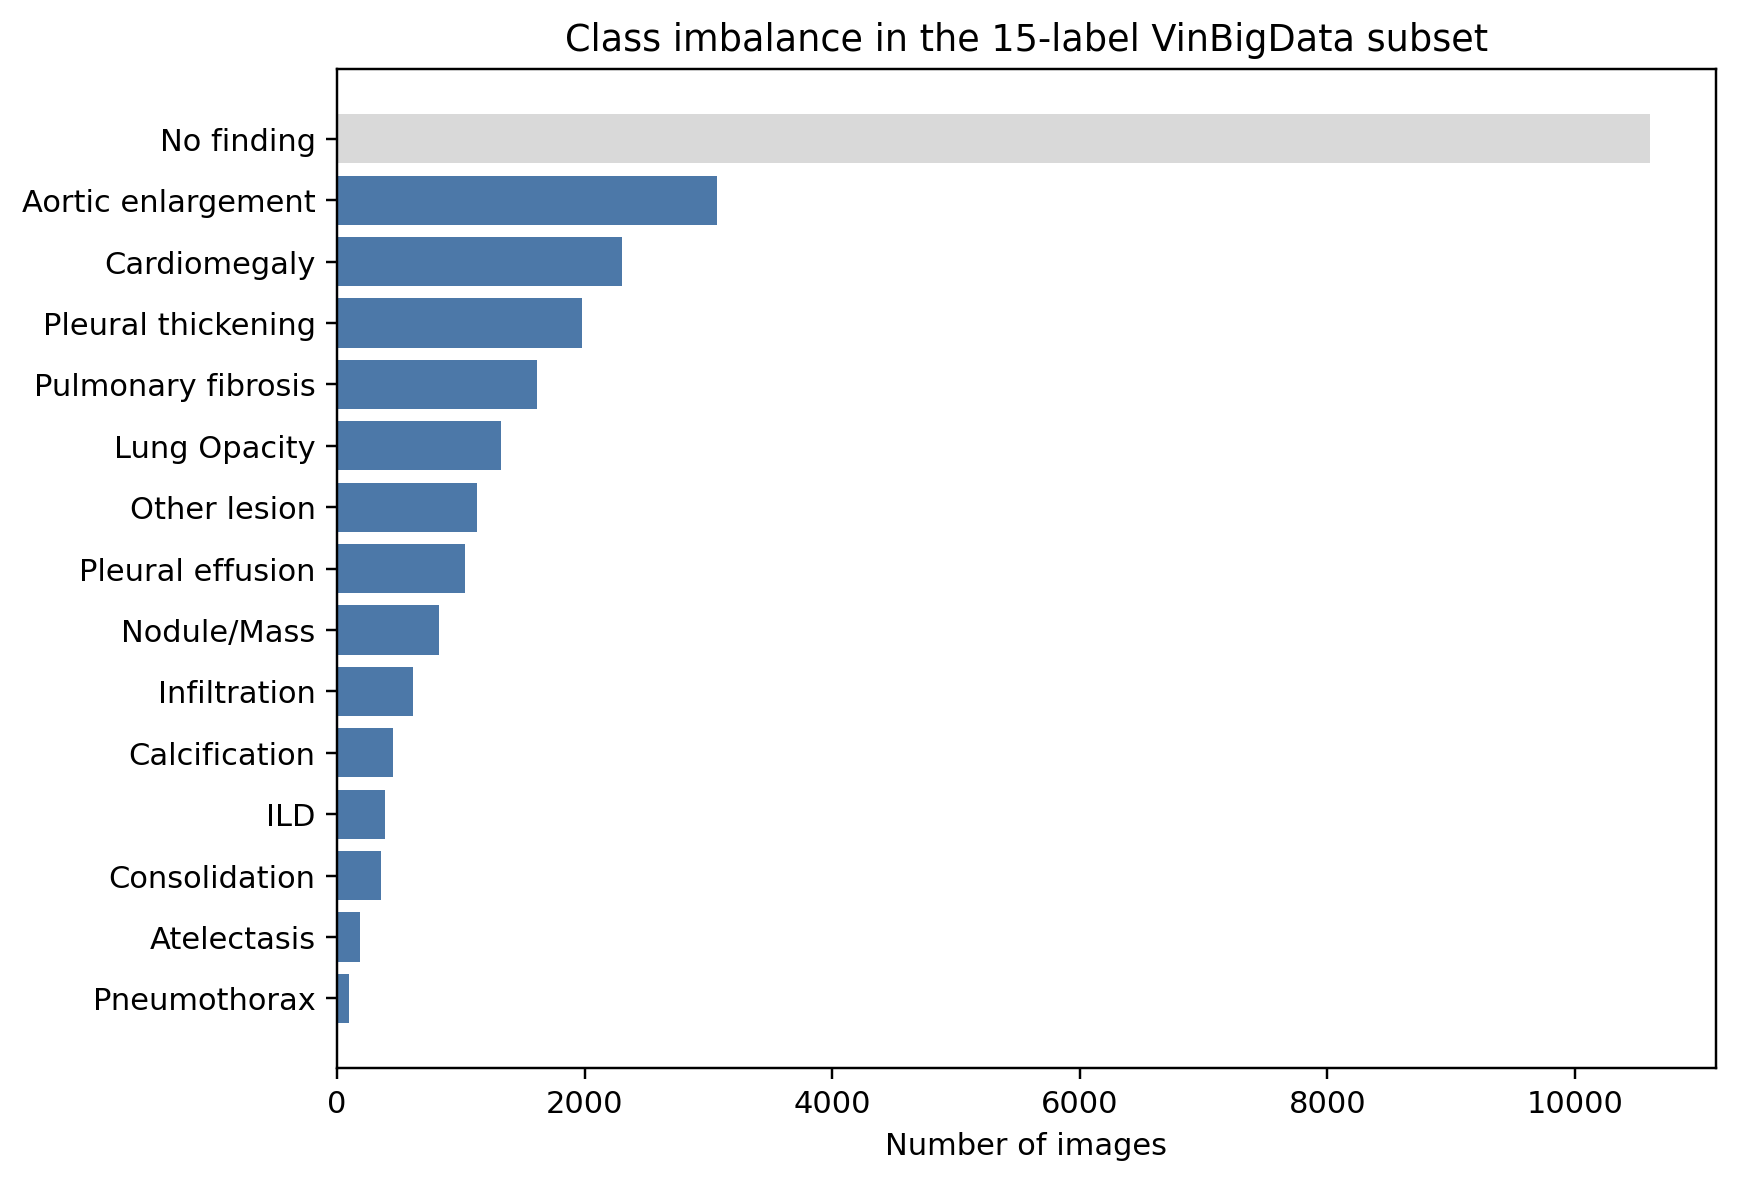
\includegraphics[width=\columnwidth]{figures/class_distribution.png}
\caption{Label frequency in the retained 15-label VinBigData subset. The dataset is strongly imbalanced, with \textit{No finding} dominating and several abnormalities occurring rarely.}
\label{fig:classdist}
\end{figure}

\section{Methods}
\subsection{Image-Level Classification}
The classification stage answers the first clinical question: \textit{which abnormalities are likely present?} All models were trained under a unified multi-label setup with input chest X-rays resized to $512\times512$, a fixed data split, and binary cross-entropy with logits as the loss function:
\begin{equation}
\begin{aligned}
\mathcal{L}_{\mathrm{BCE}} &=
-\frac{1}{NC}\sum_{i=1}^{N}\sum_{c=1}^{C}
\Bigl[
y_{ic}\log \sigma(z_{ic}) \\
&\qquad\qquad + (1-y_{ic})\log(1-\sigma(z_{ic}))
\Bigr],
\end{aligned}
\end{equation}
where $N$ is the batch size, $C=15$ is the number of labels, $y_{ic}$ is the binary ground-truth label, and $z_{ic}$ is the model logit for class $c$.

Five architectures were compared to understand the practical trade-off between transfer learning, model complexity, and classification performance in this clinical setting:
\begin{itemize}
    \item \textbf{efficientnet\_b3}: an ImageNet-pretrained EfficientNet-B3 \cite{efficientnet} with a task-specific classification head,
    \item \textbf{resnet50}: an ImageNet-pretrained ResNet-50 \cite{resnet} with a task-specific head,
    \item \textbf{vit\_base}: a Vision Transformer \cite{vit} baseline, and
    \item \textbf{swin\_base}: a hierarchical Swin Transformer \cite{swin}, whose shifted-window attention provides multi-scale feature extraction well suited to the varying spatial scales of chest X-ray abnormalities, and
    \item \textbf{simple\_cnn}: a 1.31M-parameter CNN trained from scratch, serving as a resource-constrained baseline that tests whether acceptable performance is achievable without pretrained weights or large architectures.
\end{itemize}

For transfer learning to be possible, each pretrained backbone required a small but important architectural adaptation: the original single-label classification head was removed, the final projection layer was replaced with a 15-logit output head, and the forward pass was kept in a fully multi-label setting with sigmoid activations applied only at evaluation time. In practice, this means the pretrained visual encoder is reused as a generic feature extractor while the terminal prediction layer is specialized for chest X-ray abnormalities. This comparison serves the pipeline design: the chosen classifier determines the quality of downstream reporting, so understanding how much performance depends on architecture size and pretraining is directly relevant to deployment decisions.

\subsection{Localization with YOLOv8m}
The localization stage answers the second clinical question: \textit{where is the supporting evidence?} A probability score alone does not tell the clinician which region of the image drove the prediction. YOLOv8m \cite{yolo} is trained on the VinBigData bounding-box annotations to produce spatial evidence for each detected finding. The detector is evaluated using mAP@0.5 for detection quality, and its detections are additionally converted into image-level labels so that the detector's label-level recall can be compared against the classifier. This dual evaluation quantifies both localization precision and how much clinically relevant label signal is recoverable from bounding boxes alone.

In the pipeline, YOLO is not a competing classifier. Its role is to provide confirmatory or contradictory spatial evidence that the reporting stage can reference when generating the final summary.

\subsection{Agentic Reporting Layer}
The reporting stage addresses the third clinical question: \textit{how should the evidence be organized for review?} In clinical practice, a radiologist does not hand a referring physician a list of probabilities; they produce a structured report with supported findings, uncertain observations, and an overall impression. The agentic reporting layer emulates this structure:
\begin{equation}
\begin{aligned}
\text{CXR}
&\rightarrow \text{classifier}
\rightarrow \text{detector} \\
&\rightarrow \text{agentic AI}
\rightarrow \text{structured report}.
\end{aligned}
\end{equation}

The layer consumes five inputs: (1) the full classifier probability vector, (2) thresholded predicted labels, (3) YOLO detections and their confidence scores, (4) bounding-box coordinates, and (5) explicit classifier-detector agreement or disagreement flags. From these, it generates a report containing supported findings (where both classifier and detector agree), uncertain findings (where only one source provides evidence), a short clinical impression, review guidance highlighting areas of model disagreement, and a safety statement. Architecturally, this layer follows a few explicit agentic design patterns: structured intermediate state instead of free-form prompt stuffing, provider-agnostic gateway access, schema-validated JSON outputs, deterministic decoding for reproducibility, and bounded retries when a response fails validation. These patterns matter because the reporting layer is useful only if it is inspectable and stable enough to sit on top of medical-model outputs.

To bridge the gap between low-level VinBigData labels and the broader categories a clinician uses when composing an impression, the report also maps findings into derived global buckets: \textit{No acute abnormality}, \textit{Cardiomediastinal abnormality}, \textit{Pleural abnormality}, and \textit{Chronic interstitial or fibrotic pattern}. These are interpretive summaries intended to improve readability; they are not treated as additional supervised labels. This local-versus-global distinction is central to the report design: some findings are naturally supported by boxes, while broader summary statements are derived from the total evidence bundle rather than from a single localized detection.

\section{Experimental Setup}
All training scripts use fixed defaults to ensure reproducibility. Most transfer-learning classifiers were trained for 10 epochs, which proved sufficient given their pretrained starting points, while the from-scratch CNN was trained for 100 epochs to allow convergence without pretrained initialization. A follow-up ViT-Base run was extended to 100 epochs, and we report its best validation checkpoint. All classification models used AdamW optimization with a learning rate of $10^{-4}$, weight decay of $10^{-4}$, and cosine learning rate scheduling. The primary classification metric is macro AUC-ROC. We consider it a reasonable primary metric for this setting because it is threshold-independent, gives each class equal weight despite the long-tailed frequency distribution, and prevents dominant classes such as \textit{No finding} from masking weak rare-class behavior. It is not a complete answer to class imbalance on its own, but for model selection it is sufficient as a headline metric because the pipeline's first-stage goal is robust ranking across all classes before any operating threshold is fixed. Macro F1 and exact-match style metrics are still reported downstream once thresholded decisions are required.

The YOLO localization experiments include an initial 10-epoch run and longer continuation runs; the best checkpoint is reported. All experiments were run using Pittsburgh Supercomputing Center resources with NVIDIA V100 GPUs, and the repository is structured so that any classification or localization run can be reproduced from the cleaned layout.

\section{Results}
\subsection{Image-Level Classification}
Table~\ref{tab:classification} and Fig.~\ref{fig:clfcomp} summarize the classifier comparison. The main pattern is that transfer learning clearly helps on this dataset. Swin achieves the strongest performance at 0.9665 macro AUC-ROC, followed closely by EfficientNet-B3 (0.9564) and ResNet-50 (0.9550). The best ViT-Base run improves to 0.8712 macro AUC-ROC, but it still trails the CNN and the stronger pretrained backbones, suggesting that a vanilla ViT remains a weaker fit for this dataset even with longer training.

The most practically important secondary result is the from-scratch CNN: with only 1.31M parameters, it reaches 0.9314 macro AUC-ROC. This matters because it shows that the classification stage does not strictly require a large transformer. In a resource-constrained deployment, for instance a clinic without GPU infrastructure for an 87M-parameter model, the lightweight CNN could serve as the classifier while the localization and reporting stages remain unchanged. This is a direct benefit of the modular pipeline design.

At the same time, Swin's 3.5-point advantage over the CNN shows that stronger pretraining and hierarchical multi-scale attention do yield meaningful gains when compute is available. For the remainder of the pipeline evaluation, Swin is used as the primary classifier.

\begin{table}[t]
\caption{Image-Level Classification Results on the 15-Label VinBigData Subset}
\label{tab:classification}
\centering
\footnotesize
\begin{tabular}{lccc}
\toprule
Model & Params & Epochs & Macro AUC-ROC \\
\midrule
simple\_cnn & 1.31M & 100 & 0.9314 \\
efficientnet\_b3 & 11.49M & 10 & 0.9564 \\
resnet50 & 24.56M & 10 & 0.9550 \\
vit\_base & 86.84M & 100 & 0.8712 \\
swin\_base & 87.28M & 10 & 0.9665 \\
\bottomrule
\end{tabular}
\end{table}

\begin{figure}[t]
\centering
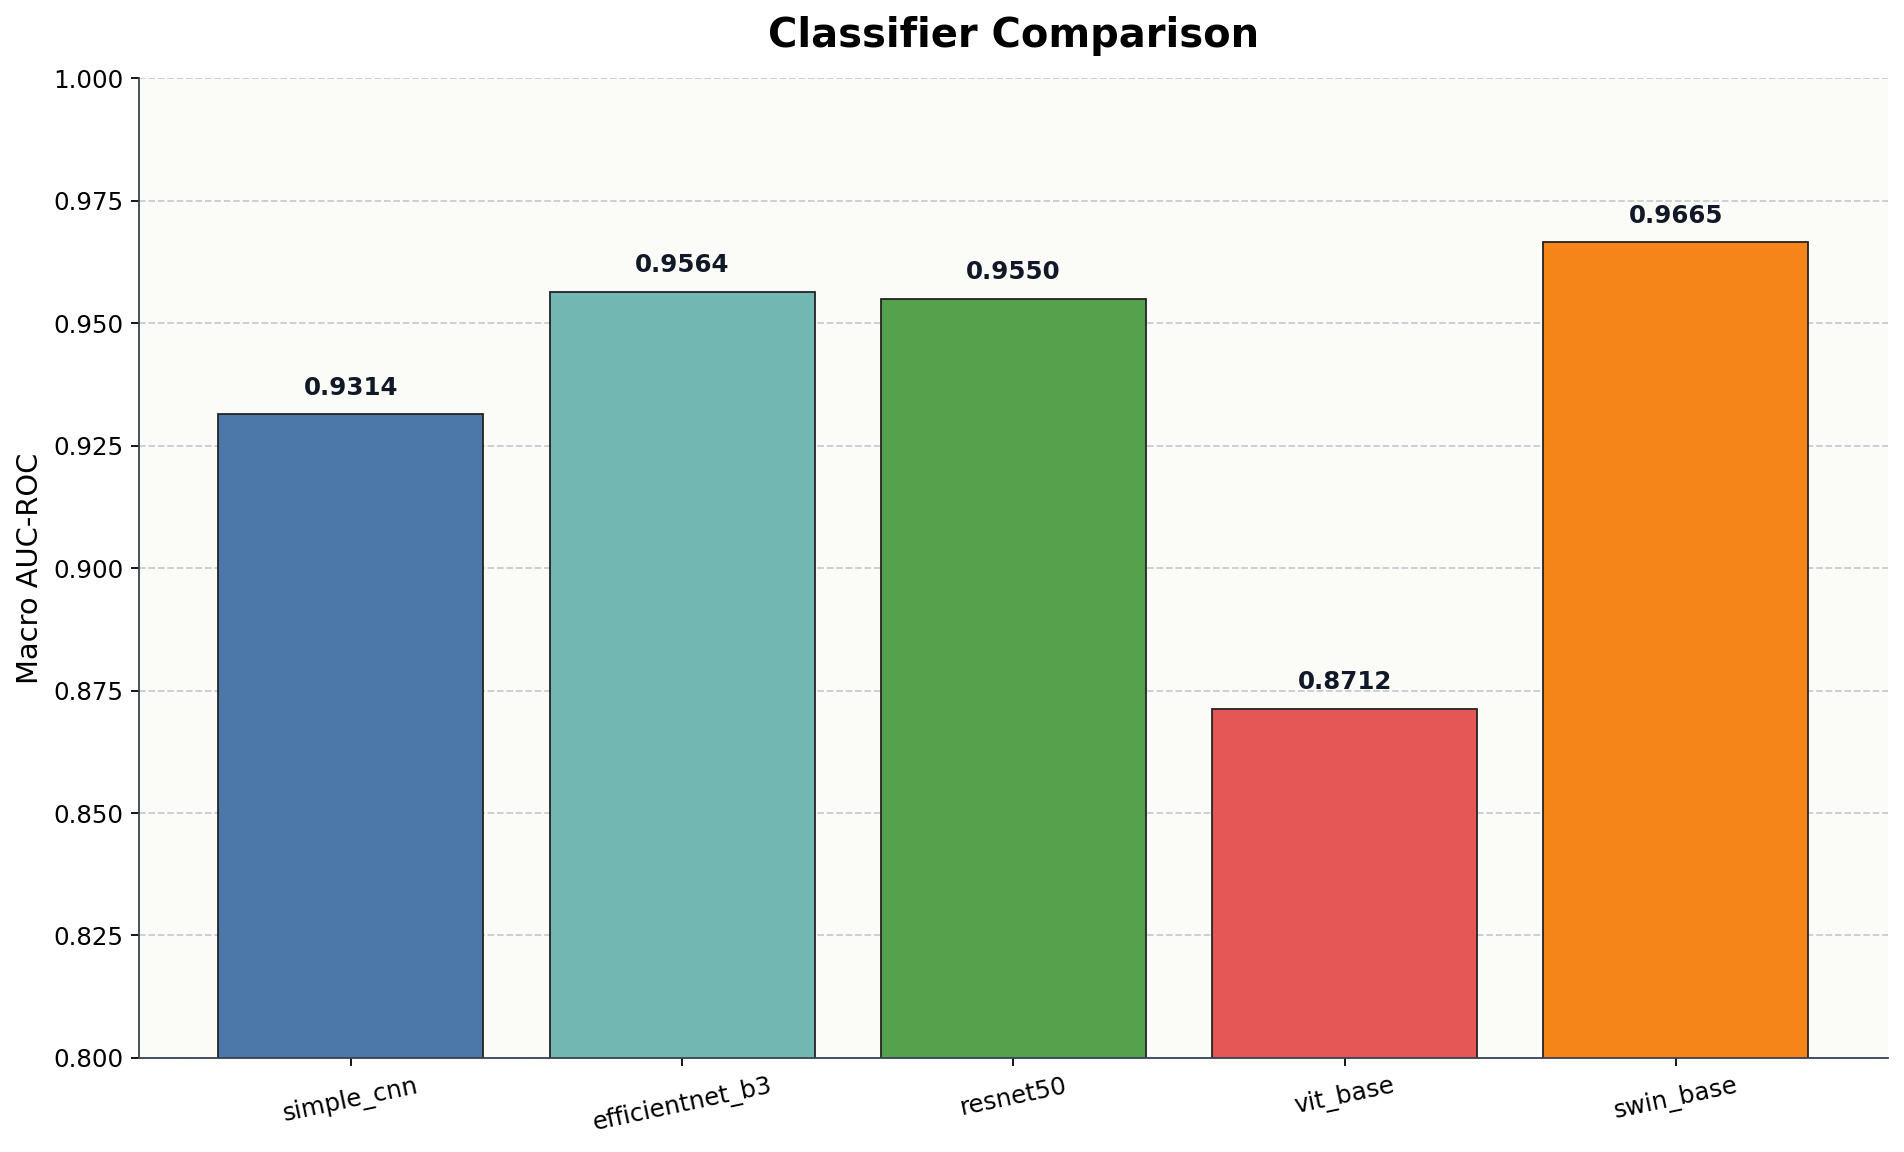
\includegraphics[width=\columnwidth]{figures/classifier_comparison.png}
\caption{Minimal comparison of the retained image-level classifiers. Transfer learning helps substantially, but the lightweight from-scratch CNN remains a strong sanity-check baseline.}
\label{fig:clfcomp}
\end{figure}

\subsection{Localization Performance}
The best YOLOv8m run reached 0.3666 mAP@0.5; a larger YOLOv8l variant did not materially improve this. The modest detection mAP is expected given the difficulty of the task because VinBigData bounding boxes include diffuse abnormalities like lung opacity and ILD, which lack the well-defined spatial boundaries that object detectors are designed for. However, detection mAP alone understates the detector's value in the pipeline. YOLO is not meant to compete with Swin on classification. Its role is to provide a second, spatially grounded evidence channel. When the classifier flags cardiomegaly and the detector draws a bounding box over the cardiac silhouette, the reporting layer can state that the finding has both image-level and localized support. When only one source provides evidence, the report marks the finding as uncertain. This agreement-disagreement signal is the main way localization contributes to clinical explainability.

\subsection{End-to-End Workflow Evaluation}
Table~\ref{tab:agentic} evaluates the complete pipeline on a 300-case review slice. The integrated workflow achieves 0.750 exact-match accuracy and 0.9560 macro accuracy, slightly exceeding both Swin alone and YOLO-derived labels on these metrics. On macro AUC-ROC, however, it reaches 0.7063, which remains below Swin's 0.7481 while improving over YOLO-derived labels at 0.6374. This pattern is consistent with the reporting layer's intended role: it is an explainability and communication module, not a new visual backbone that should be expected to outperform the strongest classifier on ranking quality.

The more informative result is the case-level breakdown. The agentic layer improved over Swin on 16 cases and over YOLO on 33 cases, while underperforming Swin on 12 cases and YOLO on 9 cases. The improvements typically occurred when one model was uncertain and the other provided supporting evidence, allowing the reporting layer to make a more informed final call. The degradations occurred when the layer inherited a confident but incorrect prediction from one upstream model and could not override it from the other. This asymmetry highlights both the value and the limitation of a fusion-based reporting approach: it can strengthen weak signals but cannot fully compensate for high-confidence upstream errors.

The stronger contribution of the reporting stage is qualitative rather than quantitative. Rather than a single label vector, the clinician receives a structured summary that states which findings are supported by both models, which are uncertain, and where the two sources disagree, information that is invisible in a raw probability output. We also performed exploratory comparisons against agentic-model alternatives, including MedGemma-style medical LLM prompting, and the main lesson was not that one model universally dominates another. Instead, the grounded pipeline consistently produced more auditable outputs because every report section is tied back to explicit classifier scores, detector boxes, and agreement logic. Medically specialized language models can phrase findings naturally, but without the same structured evidence contract they are more difficult to audit as decision-support components.

\begin{table}[t]
\caption{300-Case Comparison of the End-to-End Decision-Support Workflow}
\label{tab:agentic}
\centering
\footnotesize
\begin{tabular}{lccc}
\toprule
System & Exact-Match & Macro Acc & Macro AUC \\
\midrule
Swin classifier & 0.7400 & 0.9542 & 0.7481 \\
YOLO labels & 0.7300 & 0.9464 & 0.6374 \\
Agentic workflow & 0.7500 & 0.9560 & 0.7063 \\
\bottomrule
\end{tabular}
\end{table}

\subsection{Qualitative Reporting Scenarios}
Representative outcomes from the retained report set illustrate where the workflow is most useful in practice.

\begin{figure*}[t]
\centering
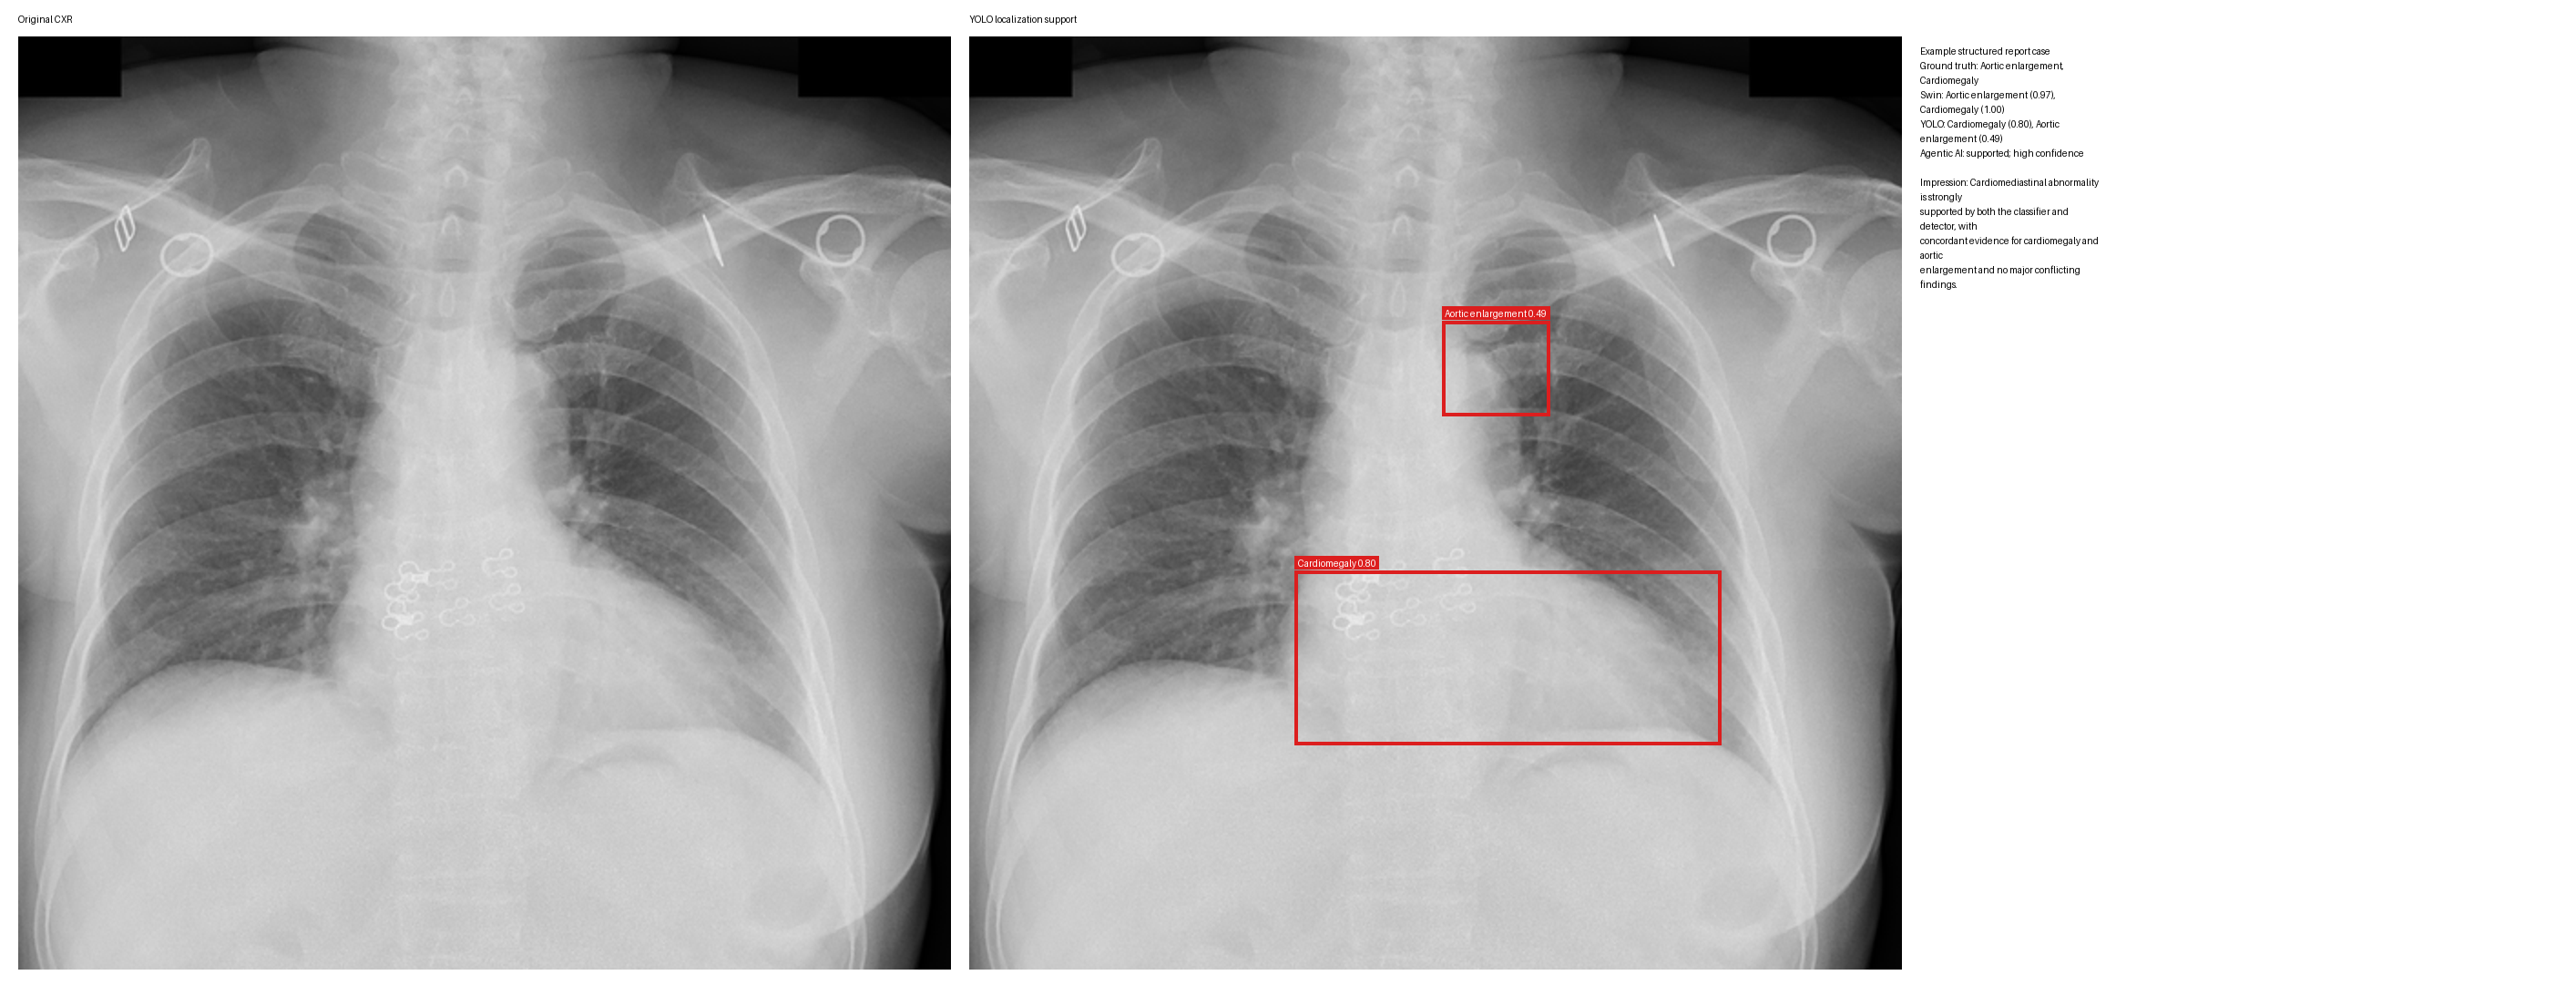
\includegraphics[width=\textwidth]{figures/example_report_case.png}
\caption{Ground-truth-versus-YOLO comparison examples. In each row, the left panel shows merged radiologist ground-truth boxes and the right panel shows YOLO predictions. Top row: a single-label case where both the ground truth and YOLO indicate \textit{Aortic enlargement}. Bottom row: a multi-label case with radiologist labels \textit{Aortic enlargement}, \textit{Cardiomegaly}, \textit{Lung Opacity}, and \textit{Nodule/Mass}; YOLO recovers the first three localizable patterns except the more diffuse \textit{Lung Opacity} finding.}
\label{fig:examplecase}
\end{figure*}

\noindent\textbf{Vanilla scenario (minimal conflict).}
In the simplest workflow setting, the classifier, detector, and ground truth all align on either \textit{No finding} or a small number of focal abnormalities. In these cases the pipeline produces a conservative summary without forcing the clinician to sift through 15 individual probability scores. This is the simplest but most common workflow scenario, and handling it efficiently matters because low-conflict cases dominate clinical volume.

\medskip
\noindent\textbf{Medium-conflict scenario.}
In moderately conflicted cases, the classifier and detector agree on the major focal abnormality but differ on one secondary or diffuse finding. The report is useful here because it does not collapse the disagreement into a single opaque output. Instead, it preserves the supported finding as ``backed by both sources'' while explicitly marking the weaker finding as uncertain. A reviewing clinician can immediately see which part of the case is stable and which part still requires visual scrutiny.

\medskip
\noindent\textbf{High-conflict scenario.}
In the hardest cases, multiple findings are present and the evidence channels diverge substantially, for example when the classifier captures diffuse disease patterns that the detector cannot localize cleanly, or when one branch overcalls a focal lesion. The reporting layer is most valuable in these high-conflict settings because it surfaces the disagreement explicitly instead of hiding it inside an aggregate metric. The final report can then distinguish findings with dual support from classifier-only or detector-only claims, which is precisely the behavior needed for a first-pass clinical review tool.

\section{Discussion}
The principal finding of this work is that the value of the pipeline lies in its workflow design rather than in any single component's performance. A radiologist reviewing a chest X-ray does not simply classify an image; they identify findings, locate supporting evidence, weigh certainty, and compose an impression. The pipeline mirrors this cognitive structure, and its clinical utility comes from making each step explicit and auditable rather than from maximizing a single metric.

This has practical implications for how such a system would be used. A clinician interacting with the pipeline sees three layers of information: which abnormalities the classifier predicts, with probabilities; where the detector places supporting bounding boxes, if any; and a structured summary that distinguishes well-supported findings from uncertain ones. If the classifier and detector disagree on a finding, the report says so. If the classifier is confident but the detector found no spatial evidence, the report marks the finding as uncertain. This transparency differs fundamentally from receiving a single probability vector, which offers no insight into why a prediction was made or how strong each source of evidence is.

The modularity of the pipeline also has deployment implications. The transfer-learning results show that pretrained backbones are the strongest default choice when compute is available, especially Swin. The CNN baseline then demonstrates that the same architecture can still be served by a model as small as 1.31M parameters without catastrophic degradation. This means the same pipeline architecture could be deployed in resource-constrained settings with a lighter classifier while keeping the localization and reporting stages intact. The choice is a deployment trade-off, not an architectural redesign.

The localization branch's modest detection mAP (0.3666) deserves honest interpretation. As a standalone detector, this performance would be insufficient for clinical reliance. But the branch is not intended to operate on its own; it serves as a confirmatory evidence channel within the report. Its primary value is for focal abnormalities (aortic enlargement, cardiomegaly, nodules) where bounding boxes correspond meaningfully to anatomical findings. For diffuse abnormalities like ILD or lung opacity, the detector is less reliable, and the pipeline handles this gracefully by reporting the finding as classifier-only.

The agentic reporting layer's quantitative contribution is modest (0.750 exact-match vs.\ Swin's 0.740), but its qualitative contribution is substantial. It transforms raw model outputs into a document that resembles the structured reporting format radiologists already use: supported findings, uncertain observations, an impression, and review guidance. The implementation also highlights a practical engineering point about provider comparison. The useful unit of comparison is not just ``which LLM writes the best prose,'' but which provider can operate reliably inside a constrained orchestration loop with schema validation, deterministic settings, and evidence-grounded prompts. In that sense, the design patterns around the agent matter as much as the model endpoint itself.

\section{Limitations}
Several limitations constrain the conclusions that can be drawn from this work. First, the study uses the public 15-label Kaggle view of VinBigData rather than the full original taxonomy, which means the pipeline has not been evaluated on every diagnostic nuance present in the broader dataset. Second, the agentic reporting layer has not been validated against radiologist-authored free-text reports in a clinical reader study; the structured summaries are evaluated against ground-truth labels, not against the nuanced language a radiologist would actually write. Third, the reporting layer inherits upstream errors; it organizes and contextualizes model outputs but cannot independently correct a confident misclassification or a missed detection. Fourth, the MedGemma and provider-level comparisons described here are exploratory rather than a fully standardized benchmark. Fifth, the analysis emphasizes aggregate metrics and does not yet include probability calibration studies, external validation on out-of-distribution data, or subgroup analyses across patient demographics.

These limitations are important for framing. The system is an explainable decision-support prototype with a reproducible code path, not a clinically deployable autonomous reporting system. Closing the gap to deployment would require prospective reader studies, calibration analysis, and validation on external datasets with different acquisition protocols and patient populations.

\section{Conclusion}
This work presents a multi-stage chest X-ray decision-support pipeline designed to bridge the gap between model output and clinical usability. The pipeline mirrors the cognitive workflow a radiologist follows: classification, localization, and structured reporting, while keeping each stage modular and auditable. Transfer-learned classifiers, especially Swin, provide the strongest image-level performance; a lightweight CNN shows that the same workflow remains viable under tighter compute constraints; YOLO contributes spatial evidence that strengthens explainability for focal findings; and the agentic reporting layer transforms raw model outputs into a structured summary that a clinician can review, question, and act on. The system is best understood not as a diagnostic model but as a first-pass assistant: a tool that organizes evidence and makes uncertainty explicit so that the clinician's review starts from a structured foundation rather than a raw probability vector.

\section*{Acknowledgment}
The author thanks the VinBigData dataset providers for releasing the chest X-ray data through an open Kaggle challenge. The author also thanks Dr.\ Newell Washburn for course guidance and Tushar Nayak for reviews and feedback on the project. Compute resources were provided by the Pittsburgh Supercomputing Center.

\begin{thebibliography}{00}
\bibitem{vinbigdata} H. Q. Nguyen et al., ``VinDr-CXR: An open dataset of chest X-rays with radiologist's annotations,'' \textit{Scientific Data}, vol. 9, no. 1, 2022.
\bibitem{chexnet} P. Rajpurkar et al., ``CheXNet: Radiologist-level pneumonia detection on chest X-rays with deep learning,'' \textit{arXiv preprint arXiv:1711.05225}, 2017.
\bibitem{pham2022vindr} H. H. Pham et al., ``An accurate and explainable deep learning system improves interobserver agreement in the interpretation of chest radiograph,'' \textit{arXiv preprint arXiv:2208.03545}, 2022.
\bibitem{swin} Z. Liu et al., ``Swin Transformer: Hierarchical vision transformer using shifted windows,'' in \textit{Proc. IEEE/CVF International Conference on Computer Vision}, 2021, pp. 10012--10022.
\bibitem{vit} A. Dosovitskiy et al., ``An image is worth 16x16 words: Transformers for image recognition at scale,'' in \textit{International Conference on Learning Representations}, 2021.
\bibitem{resnet} K. He, X. Zhang, S. Ren, and J. Sun, ``Deep residual learning for image recognition,'' in \textit{Proc. IEEE Conference on Computer Vision and Pattern Recognition}, 2016, pp. 770--778.
\bibitem{efficientnet} M. Tan and Q. Le, ``EfficientNet: Rethinking model scaling for convolutional neural networks,'' in \textit{International Conference on Machine Learning}, 2019, pp. 6105--6114.
\bibitem{yolo} G. Jocher, A. Chaurasia, and J. Qiu, ``Ultralytics YOLO,'' 2023. [Online]. Available: \url{https://github.com/ultralytics/ultralytics}
\bibitem{syedamahmood2020finegrained} T. Syeda-Mahmood et al., ``Chest X-ray report generation through fine-grained label learning,'' \textit{arXiv preprint arXiv:2007.13831}, 2020.
\bibitem{liu2021contrastive} F. Liu et al., ``Contrastive attention for automatic chest X-ray report generation,'' in \textit{Findings of ACL}, 2021.
\bibitem{najdenkoska2022uncertainty} I. Najdenkoska et al., ``Uncertainty-aware report generation for chest X-rays by variational topic inference,'' \textit{Medical Image Analysis}, vol. 82, p. 102603, 2022.
\bibitem{lee2023cxrllava} S. Lee et al., ``CXR-LLAVA: A multimodal large language model for interpreting chest X-ray images,'' \textit{arXiv preprint arXiv:2310.18341}, 2023.
\bibitem{ziegelmayer2023gpt4} S. Ziegelmayer et al., ``Evaluation of GPT-4's chest X-ray impression generation: A reader study on performance and perception,'' \textit{JMIR Medical Informatics}, vol. 25, p. e50865, 2023.
\end{thebibliography}

\end{document}
